\providecommand{\main}{../../../..}
\documentclass[\main/dresen_thesis.tex]{subfiles}

\begin{document}
  \label{sec:monolayers:nanoparticle:structuralCharacterization}
  The following paragraphs list the experimental methods, conditions and data treatment that were applied to characterize the nanoparticle batches.
  In \reftab{tab:monolayers:nanoparticles:charMethod:overview} the characterization methods applied to the different samples are summarized.

  \begin{table}[!htbp]
    \centering
    \caption{\label{tab:monolayers:nanoparticles:charMethod:overview}Summary with which methods the four nanoparticle batches are characterized.}
    \begin{tabular}{ l | l }
      \textbf{Sample} & \textbf{Characterization Methods}\\
      \hline
      Ol-CoFe-C   & TEM, XRD, EDX, SAXS, SANS(POL), VSM \\
      Ac-CoFe-C   & TEM, XRD, EDX, SAXS, SANS(POL), VSM \\
      Ac-CoFe-C-2 & TEM, XRD, EDX, SAXS, SANS(POL), VSM \\
      Ac-CoFe-C-3 & TEM, SAXS \\
      \hline
    \end{tabular}
  \end{table}

  \paragraphNewLine{Transmission Electron Microscopy}
    Transmission electron microscopy is used to visually characterize a sample of the prepared dispersion and validate the structural quality of the batch.
    For the measurement in each case a drop of a dispersion with a concentration of $c \approx 0.1 \unit{mg/mL}$ is transferred to a copper grid and measured on a Zeiss Leo 902 (\refsec{ch:instruments:laboratoryInstruments:tem}).
    The TEM micrographs are obtained with an acceleration voltage of $120 \unit{kV}$ with a \ch{LaB6} cathode in bright field mode.
    To evaluate the particle size and size distribution, the edge length of over 100 nanocubes is measured using the software Fiji \cite{Schindelin_2012_Fijia} and evaluated by fitting a log-normal distribution as described in \refsec{ch:methods:em}.

  \paragraphNewLine{X-Ray Diffraction}
    XRD of Ac-CoFe-C and Ol-CoFe-C was measured in cooperation with the group of Daniel Nižňanský from the Department of Inorganic Chemistry at the Charles University in Prague on an PANanalytical X'Pert PRO, which is described in \refsec{ch:instruments:laboratoryInstruments:xrd}.
    For the measurement, samples of the nanoparticles were dried on glass substrates.
    The diffractometer operated with a Cu-K$\alpha$ source ($\lambda \eq 1.54 \unit{\angstrom}$), and a $2 \theta \eq 5^\circ - 80^\circ$ has been measured.
    The instrumental broadening is determined from a \ch{LaB6} reference measurement (SR 660b, NIST).
    The nanoparticles from Ac-CoFe-C-2 were measured on a Huber G620 with a Mo-K$\alpha$ source ($\lambda \eq 0.71 \angstrom$) in the working group of Prof.\ Dr Mathur in the University of Cologne on a precipitated powder of the nanoparticles.
    For this instrument it was not possible to obtain a reference measurement to estimate the instrumental broadening.
    The data is analyzed using the FullProf suite \cite{Rodriguez_1993_Recen} as described in \refsec{ch:methods:xrd}.
    In all cases a LeBail refinement has been performed comparing the data to the phase of the inverse spinell structure of cobalt ferrite (space group $Fd\bar{3}m$, No. 227).
    For Ol-CoFe-C an additional phase of a w\"ustite structure is included in the LeBail refinement.
    From the refined structure, the lattice constant of the phases are determined, as well as the crystallite sizes.

  \paragraphNewLine{Energy-Dispersive X-Ray Spectroscopy}
    Using the scanning electron microscope Neon Zeiss 40 (\refsec{ch:instruments:laboratoryInstruments:sem}) EDX measurements of the nanoparticles Ac-CoFe-C, Ac-CoFe-C-2 and Ol-CoFe-C were performed.
    For the measurement, $20 \unit{\musf L}$ of a highly concentrated fraction ($c > 5 \unit{mg/mL}$ of the dispersions is drop casted on a silicon substrate with a surface area of $12.5 \unit{mm^2}$ to obtain a thick layer of nanoparticle material.
    The electron beam was accelerated with $20 \unit{kV}$ and in each case the X-ray spectrum was measured five times at different positions of the sample for a time of $2 \unit{min}$ each.
    The spectra are evaluated using the software INCA, which compares the intensity of the K-lines for each element with the literature values to extract the relative number of atoms, thereby providing the relative ratio of cobalt and iron in the samples.
    The ratios of cobalt to iron from the five measured points on the sample are averaged and the standard deviation is estimated.
    From the measured ratio $r \eq N_\mathrm{Fe} / N_\mathrm{Co}$, the number of cobalt and iron cations per formula unit are determined for the samples prepared from acetylacetonates.
    It is common in literature to assume that the formula unit has a structure of $\ch{Co_x Fe_{3-x} O4}$ \cite{Wu_2014_Monol, Sathya_2016_Cofeo}.
    For this assumption $x$ is determined by the ratio $r \eq N_{\ch{Fe}} / N_{\ch{Co}}$ by
    \begin{align}
      x \eq \frac{3}{1 + r}.
    \end{align}
    This implies an occupation of the inverse spinell lattice with both \ch{Fe^{2+}} and \ch{Fe^{3+}} for the crystal to be neutral.
    M\"ossbauer studies in literature suggest that no \ch{Fe^{2+}} is found in the acetylacetonate synthesis route, and under this assumption an alternative formulation of the formula unit is additionally followed, where vacancies are allowed in the crystal structure to obtain neutral charge.
    In this case the number of cobalt and iron cations in \ch{Co_x Fe_y O4} obey the relation
    \begin{align}
      2 x + 3 y \eq 8
    \end{align}
    for the formula unit to be neutral.
    In the limit of no cobalt in the sample ($x \eq 0$), the formula unit corresponds to maghemite and for full occupation ($x \eq 1$) it corresponds to the ideal cobalt ferrite structure described in \refsec{ch:theoreticalBackground:cobaltferrite}.
    With this relation and the ratio from EDX, the number of cobalt and iron cations in a unit cell are determined by
    \begin{align}
      x \eq \frac{8}{2 + 3r},\\
      y \eq \frac{8r}{2 + 3r}.
    \end{align}

    Given the atomic composition from EDX and the lattice constant $a$ from XRD, the density of the nanoparticles is calculated by
    \begin{align}
      \rho \eq \frac{\sum_i N_i m_i}{a^3},
    \end{align}
    where $N_i$ is the number of atoms of element $i$ in a unit cell, $m_i$ the respective atomic mass read from the periodic table of elements and $a$ the cubic lattice constant.

  \paragraphNewLine{Small-Angle Scattering}
    For the measurement of SAXS the nanoparticle dispersions are filled in borosilicate capillaries (Hilgenberg GmbH) with $1.5 \unit{mm}$ diameter and a $0.01 \unit{mm}$ wall thickness, which are sealed using a plastic stopper and glue gun.
    The used solvents and concentrations are given in \reftab{tab:monolayers:charMethod:sampleConcentrations}.
    The concentrations were roughly estimated by gravimetry, where first a container is measured empty, then the solvent in the dispersion is evaporated within the container and the weight of the particles is given by the additional mass thereafter.
    The stated mass concentration overestimates the inorganic content of the sample as organic contents in the dispersion are not removed.
    \begin{table}[!htbp]
      \centering
      \caption{\label{tab:monolayers:charMethod:sampleConcentrations}Solvents and mass concentrations $c_m$ for samples measured in SAXS and SANS.}
      \begin{tabular}{ l | l | c | l | c }
        \textbf{Sample}  & Solvent (SAXS) & $c_m^\mathrm{SAXS} \,/ \unit{gL^{-1}}$ & Solvent (SANS) & $c_m^\mathrm{SANS}\,/ \unit{gL^{-1}}$\\
        \hline
        Ac-CoFe-C   & \textit{n}-hexane   & 2.8                 & toluene-\textit{d8}       & 2.8\\
        Ac-CoFe-C-2 & toluene             & 2.0                 & toluene-\textit{d8}       & 2.0\\
        Ac-CoFe-C-3 & toluene             & 3.0                 &                           &    \\
        Ol-CoFe-C   & cyclohexane         & 2.5                 & toluene-\textit{d8}       & 6.6\\
        \hline
      \end{tabular}
    \end{table}

    The samples are measured on two sample-to-detector distances of $3.53 \unit{m}$ and $0.83 \unit{m}$ using the GALAXI instrument (\refsec{ch:lss:galaxi}) at the \textsc{Forschungszentrum J\"ulich}.
    Capillaries filled with the solvents and an empty capillary is measured under the same conditions as references for the subtraction of the background.
    The scaling to absolute units is performed according to the procedure described in \refsec{ch:methods:saxs}.

    To measure SANS and SANSPOL, part of the stock solution is dried at ambient conditions and redispersed in toluene-$\mathrm{d_8}$ to reduce the incoherent scattering coming from hydrogen atoms and to increase the contrast.
    The mass concentrations of the dispersions from gravimetry are given in \reftab{tab:monolayers:charMethod:sampleConcentrations}.
    For Ac-CoFe-C and Ac-CoFe-C-2 the same stock solution as used in SAXS was redispersed to toluene-\textit{d8}, whereas for Ol-CoFe-C a higher concentration was used.
    The small-angle neutron scattering experiments of Ac-CoFe-C and Ac-CoFe-C-2 were measured at D22 (\refsec{ch:lss:d22}) with a wavelength of $7.2 \unit{\angstrom}$ and Ol-CoFe-C on the D33 instrument (\refsec{ch:lss:d33}) with a wavelength of $6.0 \unit{\angstrom}$.
    In both cases a sample aperture of $6 \times 10 \unit{mm^2}$ is used and the samples are measured at short detector distance of $2 \unit{m}$ and a long detector distance of $8 \unit{m}$.
    For both instruments the instrumental resolution is used as provided by the GRASP software for the respective instrument.
    For SANSPOL, a magnetic field of $1.2 \unit{T}$ was applied, perpendicular to the beam and in the horizontal plane.
    To evaluate the magnetic scattering, a $20^\circ$ sector around the vertical $z$ dimension is azimuthally integrated.
    Using the GRASP software, the polarization efficiency and flipping efficiency is corrected.
    For the data measured at D22, the polarization efficiency is $84 \%$ and the flipping efficiency $93 \%$, which was determined by the use of a super mirror during the beam time.
    For D33 a polarization efficiency of $97 \%$ and a flipping efficiency of $99 \%$ is used according to the instrument specifications given by the local contact.

    The SAXS data of the nanoparticles from acetylacetonates are evaluated using a spherical (\refapp{ch:appendix:formfactors:sphereCoreshell}), cubic (\refapp{ch:appendix:formfactors:sphereCoreshell}) and a superball form factor.
    The derivation of the superball form factor is described in more detail in \refsec{sec:monolayers:nanoparticle:structuralCharacterization}.

    As figure of merit for the Levenberg-Marquardt algorithm\cite{Marquardt_1963_Analgo, Oliphant_2006_Guide}, a modified $\chi^2$ on the logarithmic scale is used, which is defined by
    \begin{align}
      \chi^2 \eq \frac{1}{N-p} \sum_{i\eq 1}^{N} \frac{(\log(I_i) - \log(I_\mathrm{model}))^2}{\sigma_i^2} I^2_i
    \end{align}

    To constrain parameters of the models, the scattering length density of the nanoparticle cores is determined using the lattice parameter $a$ from XRD and the average atomic composition determined from EDX by
    \begin{align}
      \label{eq:monolayer:charMethod:calcSLD}
      \rho^\mathrm{X-ray}_\mathrm{inv. spinell}   &\eq 8 r_e \frac{N_\mathrm{Co} f_\mathrm{Co} + N_\mathrm{Fe} f_\mathrm{Fe} + 4 f_\mathrm{O}}
                                                                  {a_\mathrm{inv.\,spinell}^3},\\
      \rho^\mathrm{neutron}_\mathrm{inv. spinell} &\eq 8 \frac{N_\mathrm{Co} b_\mathrm{Co} + N_\mathrm{Fe} b_\mathrm{Fe} + 4 b_\mathrm{O}}
                                                                  {a_\mathrm{inv.\,spinell}^3},\\
      \rho^\mathrm{X-ray}_\textsf{w\"ustite}      &\eq 4 r_e \frac{N_\mathrm{Co} f_\mathrm{Co} + N_\mathrm{Fe} f_\mathrm{Fe} + f_\mathrm{O}}
                                                                  {a_\textsf{w\"ustite}^3},\\
      \rho^\mathrm{neutron}_\textsf{w\"ustite}    &\eq 4 \frac{N_\mathrm{Co} b_\mathrm{Co} + N_\mathrm{Fe} b_\mathrm{Fe} + b_\mathrm{O}}
                                                              {a_\textsf{w\"ustite}^3}.
    \end{align}
    Here, $f$ is the element specific atomic form factor for X-ray scattering and $b$ the element specific nuclear scattering length, which are  tabulated in \reftab{tab:monolayers:charMethod:scatteringLenghts} \cite{Sears_1992_Neutr, BerkeleyLab_1993_asf}.
    The constant $r_e \eq 2.8179 \unit{fm}$ is the classical electron radius.
    The numerical value $Z \eq 8$ accounts that one unit cell contains eight formula units of $\ch{Co_xFe_yO4}$ in an inverse spinell phase.
    The atomic form factor depends on the X-ray wavelength, the given values are for the wavelength of $\lambda \eq 1.3414 \unit{\angstrom}$ (wavelength used at the GALAXI instrument).
    For Ac-CoFe-C-3 no XRD was performed and therefore the literature value of the lattice constant is assumed.
    \begin{table}[ht]
      \centering
      \caption{\label{tab:monolayers:charMethod:scatteringLenghts}The real part of the atomic form factor $f$ (at $\lambda \eq 1.3414 \unit{\angstrom}$) and the nuclear coherent scattering length $b$ for the elements of the nanoparticles to determine their scattering length densities \cite{Sears_1992_Neutr, BerkeleyLab_1993_asf}.}
      \begin{tabular}{ c | l | c }
                  & $f$       & $b \, / \unit{fm}$ \\
        \hline
        $\ch{O}$  & 8.04077   & 5.803   \\
        $\ch{Co}$ & 26.3717   & 2.49  \\
        $\ch{Fe}$ & 25.7468   & 9.45  \\
        \hline
      \end{tabular}
    \end{table}

    For Ol-CoFe-C the superball form factor is used with an core-shell structure to account for the w\"ustite / inverse spinell structure of the particles and to determine the shell scattering length density $\rho_\mathrm{shell}$ and shell thickness $D_\mathrm{shell}$.
    For the SANS models, an additional oleic acid surfactant shell with the same superball parameters as the core model and a thickness $D_\mathrm{OA}$ is added to the model, which is neglected for SAXS models due to the poor contrast of oleic acid and solvent.
    The composition of the core and shell can not be determined by XRD and EDX alone as the complex structure leaves too many variables.
    There is luckily a significant contrast between the w\"ustite SLD ($\rho_\mathrm{el}^\textsf{w\"ustite} \approx 50 \cdot 10^{-6} \angstrom^{-2}$) and inverse spinell SLD ($\rho_\mathrm{el}^\mathrm{inv.\, spinell} \approx 42 \cdot 10^{-6} \angstrom^{-2}$) for X-rays, that enables to determine the relative core and shell thickness.
    And furthermore neutrons are highly sensitive to the relative iron and cobalt amount in a phase, as can be seen from \reftab{tab:monolayers:charMethod:scatteringLenghts}, which can be utilized to measure the relative composition.
    Thus the combination of SAXS and SANS can be used as a tool to solve both the core-shell structure and the compositions.

    Therefore, a parameter is introduced in the model for Ol-CoFe-C for the cobalt content $x$ from the cobalt ferrite shell \ch{Co_x Fe_{3-x} O4}.
    Using this parameter, the scattering length density of the core and shell in Ol-CoFe-C is determined by fixing the ratio of iron and cobalt $r$ to the value obtained from EDX.
    The composition of the w\"ustite phase \ch{Fe_y Co_{1-y} O} is calculated using the volume of the spinell phase $V_\mathrm{inv.\,spinell}$ and the volume of the w\"ustite phase $V_\textsf{w\"ustite}$ in the core-shell particle, as well as the lattice constants determined from XRD $a_\mathrm{inv.\,spinell}$ and $a_\textsf{w\"ustite}$.
    For this purpose the ratio $r$ that is given by
    \begin{align}
      \begin{split}
        r &\eq \frac{N_\mathrm{Fe}^\mathrm{inv.\, spinell} + N_\mathrm{Fe}^\textsf{w\"ustite}}
                    {N_\mathrm{Co}^\mathrm{inv.\, spinell} + N_\mathrm{Co}^\textsf{w\"ustite}} \\
          &\eq \frac
                 {8 (3-x) \frac{V_\mathrm{inv.\,spinell}}{a_\mathrm{inv.\,spinell}^3} +
                  4 y \frac{V_\textsf{w\"ustite}}{a_\textsf{w\"ustite}^3}}
                 {8 x \frac{V_\mathrm{inv.\,spinell}}{a_\mathrm{inv.\,spinell}^3} +
                  4 (1-y) \frac{V_\textsf{w\"ustite}}{a_\textsf{w\"ustite}^3}},
      \end{split}
    \end{align}
    is solved for the w\"ustite composition parameter $y$ by
    \begin{align}
      y &\eq \frac{2}{\nu} x + \frac{r \nu - 6}{\nu (1 + r)},\\
        & \textsf{where\,} \hspace{0.5cm} \nu \eq \frac{V_\textsf{w\"ustite}}{V_\mathrm{inv.\,spinell}} \biggl( \frac{a_\mathrm{inv.\,spinell}}{a_\textsf{w\"ustite}} \biggr)^3.
    \end{align}
    The volumes of the two phases are determined from the particle size, shell thickness and superball exponent on the fly during the fitting process, such that y is readily determined with varied particle dimensions and cobalt content in \ch{Co_x Fe_{3-x}O4}.
    % As SAXS is also sensitive to the difference of the nanoparticle core and shell size due to a stronger contrast between w\"ustite and spinell phase, the data sets for SAXS and SANS are fitted simultaneously.
    By this method, the combination of SAXS and SANS on Ol-CoFe-C provides the means to determine the particle size and size distribution, the individual core and shell thickness and atomic composition of the two phases, while being self-consistent with EDX and XRD results.

    The scattering length density of the oleic acid shell is fixed in every SANS model to the value value calculated for bulk oleic acid
    \begin{align}
      \rho^\mathrm{X-ray}_\mathrm{oleic\,acid} &\eq 8.52 \cdot 10^{-6} \angstrom^{-2},\\
      \rho^\mathrm{neutron}_\mathrm{oleic\,acid} &\eq 0.078 \cdot 10^{-6} \angstrom^{-2},
    \end{align}
    which assumes a density of $0.895 \unit{g\,mL^{-1}}$ for the oleic acid.
    The solvent scattering length densities are fixed to the values calculated from literature
    \begin{align}
      \rho^\mathrm{X-ray}_{n\mathrm{-hexane}}    &\eq 6.46 \cdot 10^{-6} \angstrom^{-2},\\
      \rho^\mathrm{X-ray}_\mathrm{toluene}       &\eq 8.01 \cdot 10^{-6} \angstrom^{-2},\\
      \rho^\mathrm{X-ray}_{\mathrm{cyclohexane}} &\eq 7.55 \cdot 10^{-6} \angstrom^{-2},\\
      \rho^\mathrm{neutron}_\mathrm{toluene-d8}  &\eq 5.66 \cdot 10^{-6} \angstrom^{-2},
    \end{align}
    where a density of $0.655 \unit{g\,mL^{-1}}$ is used for $\mathit{n}$-hexane, $0.867 \unit{g\,mL^{-1}}$ for toluene, $0.779 \unit{g\,mL^{-1}}$ for cyclohexane, and $0.943 \unit{g\,mL^{-1}}$ for toluene-d8.

    \begin{figure}[tb]
      \centering
      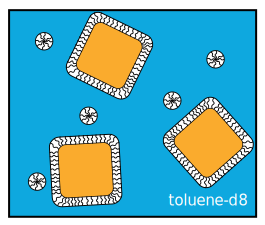
\includegraphics{monolayer_sans_superball_OA_model}
      \caption{\label{fig:monolayers:charMethods:SANSModel}Depiction of the model used for SANS: A combination of nanoparticles and oleic acid micelles. Orange is the nanoparticle material, white with curly lines the oleic acid and blue the solvent.}
    \end{figure}

    Due to the stronger contrast of oleic acid and the solvent for neutrons, oleic acid micelles in the solution become visible.
    Also it is possible that a incoherent background might be present due to the hydrogen of the oleic acid (\ch{C18H34O2}), as to why an additional constant background term is added to the model.
    The SANS data is thus described by a sum of the intensity calculated for the superball, the intensity of a spherical form factor and a constant term
    \begin{align}
      I(q) \eq I_\mathrm{superball}(q) + I_\mathrm{sphere}(q) + I_\mathrm{bg},
    \end{align}
    which is depicted in \reffig{fig:monolayers:charMethods:SANSModel}.
    The micelles introduce $r_\mathrm{OA}$ and $n_\mathrm{OA}$ as additional parameters to the model, which describe the size of the micelles and their number density in dispersion.

    To interpret particle number densities $n$, they are transformed to a mass concentration by
    \begin{align}
      c_m \eq n \rho V_p,
    \end{align}
    using the particle volume $V_p$ and the mass density of the material $\rho$.
    For the oleic acid micelles the volume fraction
    \begin{align}
      c_V \eq n V_p,
    \end{align}
    is given instead as it is the more natural to the liquid state of oleic acid.

  \paragraphNewLine{Vibrating Sample Magnetometry}
    The macroscopic magnetization of the nanoparticles Ac-CoFe-C, Ac-CoFe-C-2 and Ol-CoFe-C was measured using the PPMS Evercool II (\refsec{ch:instruments:laboratoryInstruments:vsm}).
    To obtain the magnetization in a non-interacting state at room temperature, two approaches are considered.
    In the first, $40 \unit{\musf L}$ of the nanoparticle dispersion are sealed in a vial as described in \refsec{ch:instruments:laboratoryInstruments:vsm}.
    The vial is fixed within a drinking straw, using additional folded straws to render the vial immobile.
    A moving liquid sample is a difficult system in the framework of vibrating sample magnetometry as due to air gaps the liquid is still able to move within its container during the vibration, which can lead to a systematic error in the measured signal \cite{Boekelheide_2016_Artif}.
    Therefore, in a second approach, the nanoparticle dispersion is quickly drop casted in a diluted concentration ($c \eq 0.1 \unit{mg/mL}$) on a silicon substrate using $\textit{n}$-hexane as solvent to measure the nanoparticles in a dry state for comparison.
    The background of the silicon substrate and sample holder is subtracted in this case by the measurement of an empty silicon wafer with approximately the same mass.

    For both approaches hysteresis curves are measured at $10 \unit{K}$ and $300 \unit{K}$.
    Before each measurement, a touchdown procedure is performed with the sample rod, to correct for thermal expansion due to the temperature changes.
    Each hysteresis is measured in sweep mode with a rate of $5 \unit{mT \, s^{-1}}$.
    Additionally, for the dry particles on a substrate, zero-field-, field-cooled warming curves are measured at a field of $10 \unit{mT}$ for a temperature range from $10 \ldots 350 \unit{K}$ with a heating rate of $1.5 \unit{K \, min^{-1}}$.
    For Ac-CoFe-C-2 no measurement of the dry particles has been performed.

    Using the liquid dispersion in the vial measurement, a Langevin behaviour with excess susceptibility is fit in the range from $\pm 2 \unit{T}$ to determine the magnetic moment of the non-interacting nanocubes (\refsec{ch:methods:vsm}).
    The magnetization data is scaled such that the saturation magnetization is given by the ratio of the single-particle moment and nanocube volume
    \begin{align}
      M_s \eq \frac{\bar{\mu}}{V_p}.
    \end{align}
    The average particle volume is hereby taken from the previously obtained SAXS data evaluation.

    The measurements in the dry state on a substrate are scaled to their saturation value and compared to the dispersion measurements.
    As the temperature-dependent magnetization of the liquid dispersions showed in all cases a jump in a order of magnitude upon freezing, the rescaling of the dispersion $10 \unit{K}$ is not straight forward.
    As an increase in the spontaneous magnetization value is still expected for lower temperatures, the observed increase for the dry nanocubes on the substrate is used to rescale the dispersion at $10 \unit{K}$.

    Furthermore, the temperature-dependent magnetization of the dried nanocubes on the substrate is measured after zero-field cooling and field cooling at a magnetic field of $10 \unit{mT}$.
    From the maximum of the zero-field cooled curve, the blocking temperature of the nanocubes is estimated.
\end{document}